
%---- Created by: Sinchiguano Cesar. El Carmen - June 2022 --
\documentclass[xcolor=dvipsnames,envcountsect]{beamer}
%Default package loading
\usepackage{import}
\import{sourceFile/}{source.tex}
\usepackage{graphicx}
\usepackage{caption}
\usepackage{subcaption}

%--------- START DOCUMENT ------------------
\begin{document}
\begin{frame}{\titlepage}\end{frame}
\begin{frame}{\frametitle{Contenido}\tableofcontents}\end{frame}


\section{Perfil del docente}
\begin{frame}
	\frametitle{Perfil del docente}
		\justifying
		
\begin{figure}
     \centering
     \begin{subfigure}[b]{0.3\textwidth}
         \centering
         
\includegraphics[width=\textwidth]{Figures/epn.jpg}
         %\caption{$y=x$}
         %\label{fig:y equals x}
     \end{subfigure}
     \hfill
     \begin{subfigure}[b]{0.3\textwidth}
         \centering
         
\includegraphics[width=\textwidth]{Figures/cvut.jpg}
         %\caption{$y=3sinx$}
         %\label{fig:three sin x}
     \end{subfigure}
     \vfill
     \begin{subfigure}[b]{0.2\textwidth}
         \centering
         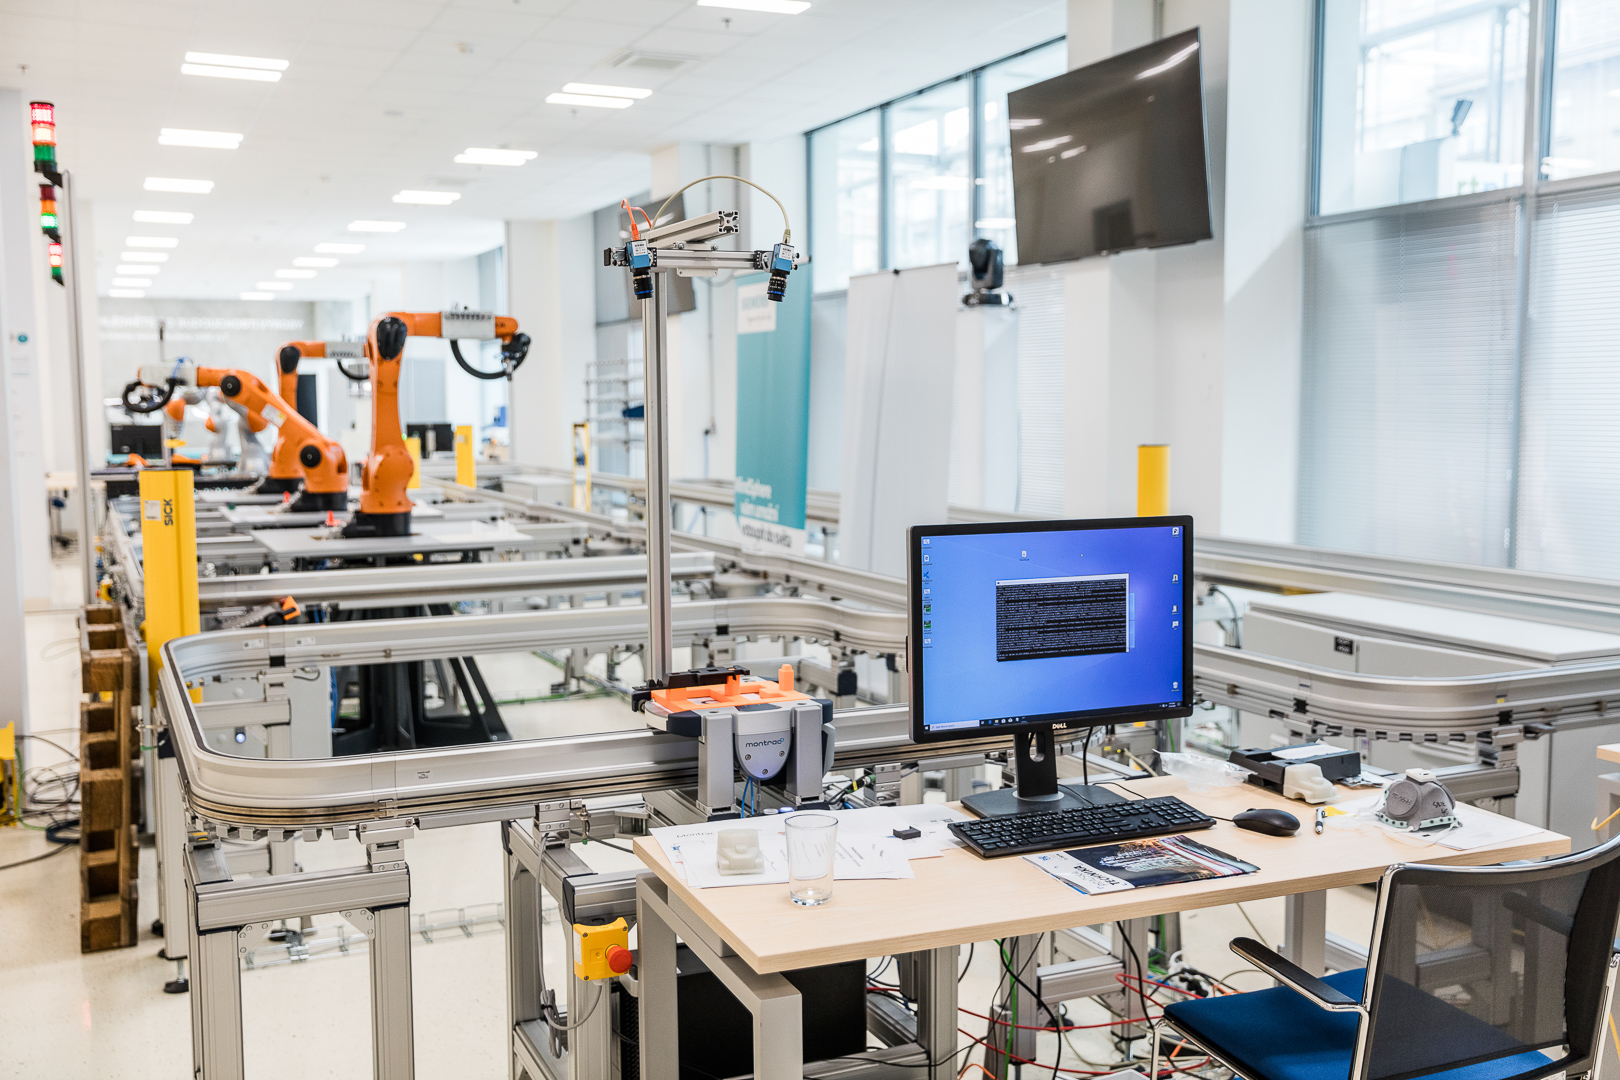
\includegraphics[width=\textwidth]{Figures/ciirc.jpg}
         %\caption{$y=5/x$}
         %\label{fig:five over x}
     \end{subfigure}
        %\caption{Three simple graphs}
        %\label{fig:three graphs}
\end{figure}



\end{frame}



%---------
\section{Consideraciones generales}
\begin{frame}
	\frametitle{Consideraciones generales}
		\justifying

\end{frame}






%---------
\section{ Sílabo}
\section{Magnitudes y unidades eléctricas}
\begin{frame}
	\frametitle{Magnitudes y unidades eléctricas}
		\justifying
		\begin{enumerate}
		\item Conceptualización de las magnitudes utilizadas en los circuitos eléctricos y electrónicos.
		\item Diferencia de potencial y tensíon.
		\item Itensidad de corriente eléctrica.
		\item Resistencia eléctrica.
		\item Potencia eléctrica.
		\item Energía eléctrica.
		\item Unidades eléctricas y equivalencias
		\end{enumerate}
\end{frame}



%---------- 
\section{Circuitos eléctricos}

\begin{frame}
		\frametitle{Circuitos eléctricos}
		\begin{enumerate}
		\item ¿Qué es un circuito elétrico?.
		\item Partes de un circuito eléctrico.
		\item Símbolos eléctricos.
		\end{enumerate}				
\end{frame}


%----------- MAIN RESULTS ------------------------------
\section{Tipos de circuitos}
\begin{frame}{Tipos de circuitos}
		\begin{enumerate}
		\item Circuito en serie.
		\item Circuito en paralelo.
		\item Circuito mixtos o serie-paralelo.
		\item Circuitos elétricos en corriente alterna.
		\end{enumerate}		
\end{frame}



%---------- 
\section{Circuitos electrónicos}
\begin{frame}
	\frametitle{Circuitos electrónicos}
	\justifying
		\begin{enumerate}
		\item ¿Qué son los circuitos electrónicos?.
		\item Tipos de circuitos electrónicos.
			\begin{enumerate}
			\item Circuitos analógicos.
			\item Circutios digitales.
			\item Circuitos mixtos.
			\end{enumerate}
		\item ¿Cómo funcionan los circuitos electrónicos?.
		\end{enumerate}		

\end{frame}


%--------- THANK YOU Text --------------------------
	\begin{frame}
		\centering
		\begin{block}
			\scshape
				\begin{center}
					\Huge\emph{Gracias!}
				\end{center}
		\end{block}
	\end{frame}
%----------------------------------------------------
\end{document}
